% !TEX root =  paper.tex
\section{Introduction}
Web accessibility is the notion of implementing web apps  
in a fashion that allows programmatic access to 
software functionalities that are otherwise only 
perceivable through certain senses (e.g., visually). 
Accessibility has been sometimes dealt with as an 
afterthought or a nice to have optional feature, 
with many developers and companies 
ignoring it altogether \cite{vendome2019can,harper2012web}. 
However, as shown in Figure \ref{fig:population-plot}, millions 
of people around the globe have software-relevant disabilities and are impacted by web accessibility, or the lack thereof. 

Furthermore, accessibility is increasingly becoming a legal 
requirement ratified into laws in many countries.
For instance, in the United States, the Americans with Disabilities Act~\cite{law:ada} 
requires all government and public agencies, as well as certain businesses, 
to make all their software and information technology 
services accessible. 
Similar provisions are required by law under the European
Union's Web Accessibility Directive \cite{law:eu_accessibility}.
Figure \ref{fig:lawsuits-plot} shows the increasing number of lawsuits
filed in federal US courts against businesses for failing to provide 
accessibility accommodations.

Despite the increasing legal, economical, and human costs due to lack of 
accessibility, there has been little work in the 
software engineering research community to automate accessibility testing.
Eler et al.~\cite{eler2018automated} check for missing attribute fields or 
incorrect attribute values related to accessibility of web pages, an approach that is 
also used in a few patents~\cite{sap2019accessibility, breeds2014software}.
The bulk of existing work focuses on topics such as 
evaluating best practices for conducting empirical accessibility evaluations, 
such as manual checklist walkthroughs~\cite{braga2014applying} or enlisting
visually-impaired users as part of user studies~\cite{bayer2006accessibility}.
A number of open-source tools have been developed to conduct simple syntactic accessibility tests 
that only check a few attribute values in a web page. 
In an audit of 13 of such accessibility testing tools conducted by the United Kingdom
Government's Office of Digital Services~\cite{ukgov:audit:2018}, 
these tools found only 26\% of a known small set of accessibility violations
present in tested web pages.

\begin{figure}%[b]
	\centering
	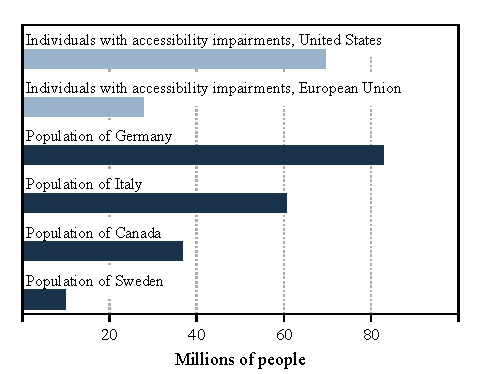
\includegraphics[width=0.70\columnwidth,height=6.0cm]{accessibility_testing/figures/population-plot}
	% \hspace{1cm}
	\caption{Number of people with software-related disabilities in the United States
		and the European Union. 
		% To put the numbers in perspective, the number of people with impairments is
		% comparable to the population of entire countries. 
		(Data compiled from: \cite{stats:accessibility_population:US, stats:accessibility_population:EU})}
	\label{fig:population-plot}
\end{figure}

The aforementioned tools are based on conducting \emph{syntactic} checks, 
which are simple markup rules (e.g., any \code{a} element must contain a non-empty string) 
to check for a minimal level of accessibility. 
However, none of the aforementioned tools analyze key accessibility 
requirements related to the \emph{semantics} of a page, such as the high level page 
structure and the roles or purpose of various elements. 
It is these semantic aspects of a page that users with 
disabilities rely on the most while using web pages~\cite{2019users_survey}, but none 
of the existing tools test for. 
Accordingly, the high level semantic analysis of web accessibility has remained 
a manual and laborious time consuming process~\cite{bai2016evaluation,
acosta2018toward,brajnik2008comparative,abou2008web}.  
   
To that end, we propose an approach that 
automates testing of a subset of web accessibility 
requirements pertaining to high level 
semantic checks that have not been amenable to automation. 
The approach is based on a visual analysis of the web page, 
coupled with a few natural language processing (NLP) steps, 
to conduct a semantic analysis of web pages. 
This analysis first identifies major cohesive regions of a 
page, then infers their 
\emph{semantic role} or purpose within the page.
Subsequently, a conformance check is conducted that determines 
whether the markup of the page correctly corresponds to the inferred semantics.  
If the markup contains the same semantic information perceivable by sighted users, 
the page is deemed accessible. Otherwise, if semantic information of the page is 
perceivable only visually but not conveyed in the markup, 
the page would be flagged as failing the accessibility test 
and the specific reasons are reported.   
In this work, we focus on vision disabilities as opposed to other forms 
of disability (e.g., hearing). The rationale for this is twofold. 
First, the web is predominantly a visual medium where most of the 
information is accessed visually as opposed to other senses. 
Second, surveys have shown that vision disabilities are the most relevant 
to web users with disabilities~\cite{2019users_survey}.

This chapter makes the following main contributions:
\begin{itemize}
    \item A novel approach for automatically testing semantic accessibility 
    requirements, which is the first to address this issue, to the best of our knowledge.
	\item An implementation of our approach, available in a tool called \toolname.
    \item A qualitative and quantitative evaluation of \toolname in terms of its 
    inference accuracy and ability to detect accessibility failures. 
    The results show that it achieves an F-measure (harmonic average of precision and recall) of 87\% for inferring semantic groupings, and is able to detect accessibility failures with 85\% accuracy. 
\end{itemize}


\begin{figure}%[b]
	\centering
	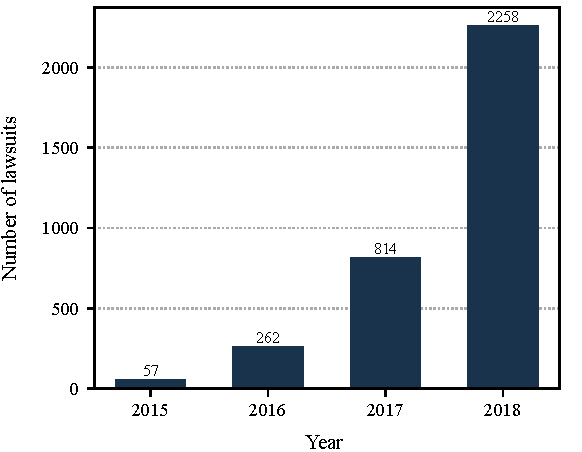
\includegraphics[width=0.70\columnwidth,height=6.0cm]{accessibility_testing/figures/lawsuits-plot}
	\caption{Number of software accessibility lawsuits filed in US federal courts per year. The number of lawsuits increased by around 3800\% over the four-year period 2015-2018. (Data compiled from: \cite{stats:accessibility_lawsuits:US_1, stats:accessibility_lawsuits:US_2})}
	\label{fig:lawsuits-plot}
\end{figure} 